% Saberes básicos (LOMLOE) asociados a esta unidad
%
% Bloque B. La materia
%   - Experimentos relacionados con los sistemas materiales: conocimiento y descripción de sus
%     propiedades, su composición y su clasificación. Técnicas de separación de mezclas.
%     Justificación: la unidad dedica una sección completa a los métodos de separación de
%     mezclas heterogéneas y homogéneas (tamizado, filtración, decantación, centrifugación,
%     extracción con disolvente, separación magnética, evaporación/cristalización, destilación
%     y cromatografía), con ejemplos y aplicaciones cotidianas (desalinización, depuradoras...).
%
% Bloque E. El cambio
%   - Los sistemas materiales: análisis de los diferentes tipos de cambios que experimentan,
%     relacionando las causas que los producen con las consecuencias que tienen.
%     Justificación: se distingue de forma explícita entre cambios físicos y químicos, con
%     ejemplos, criterios y evidencias observables para reconocerlos.
%
%   (Las reacciones químicas, la conservación de la masa y los factores que afectan a las
%    reacciones están en la Unidad 6, Chemical Reactions.)

\spacing{1.3}
\raggedbottom % pages with large figures end where the text ends (no stretched gaps between boxes)

\section{Physical and chemical changes}

\subsection{Physical changes}

\begin{definition}[Physical change]
    A change in which \textbf{no new substances} appear: the substance has the same chemical formula before and after.
\end{definition}

\begin{figure}[H]
    \centering
    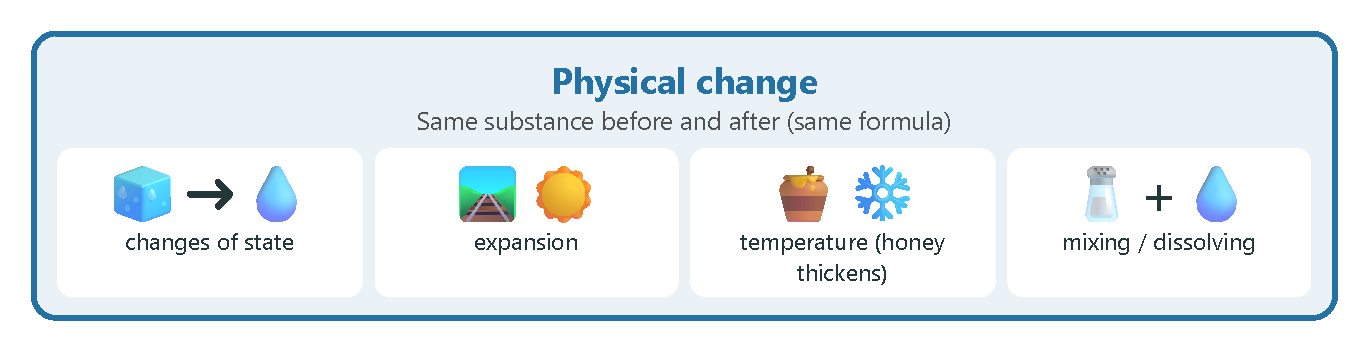
\includegraphics[width=0.85\textwidth]{FigurasSVG/Unit_5_Change_of_Matter/pdf/physical_change.pdf}
    \caption{Examples of physical changes: the substance is the same before and after.}
    \label{fig:u5_physical_change}
\end{figure}

\begin{itemize}
    \item \negsubro{Changes of temperature}: honey flows more easily when warm, but it is still honey.
    \item \negsubro{Changes of state}: ice, liquid water and water vapour are all \ch{H2O}.
    \item \negsubro{Expansion and contraction}: a metal expands when heated, but it is the same metal.
    \item \negsubro{Mixing}: iron and sulphur powder mixed together are still iron and sulphur; a magnet can separate them again.
\end{itemize}

\begin{exercise}
    Classify each physical change according to the four types above (change of temperature, change of state, expansion/contraction, mixing): a railway track on a hot day; freezing water to make ice cubes; mixing flour and sugar; honey thickening in winter.
    \begin{solu}
        Railway track: \textbf{expansion}. \\
        Ice cubes: \textbf{change of state}. \\
        Flour and sugar: \textbf{mixing}. \\
        Honey in winter: \textbf{change of temperature} (it becomes more viscous).
    \end{solu}
\end{exercise}

\begin{exercise}
    Explain why dissolving salt in water is a physical change, even though the salt seems to disappear.
    \begin{solu}
        No new substance is formed: the salt is still \ch{NaCl} and the water is still \ch{H2O}, only mixed. We can get the salt back unchanged just by evaporating the water.
    \end{solu}
\end{exercise}

\subsection{Chemical changes}

\begin{definition}[Chemical change]
    A change in which \textbf{new substances} appear, with a different formula and different properties.
\end{definition}

\begin{figure}[H]
    \centering
    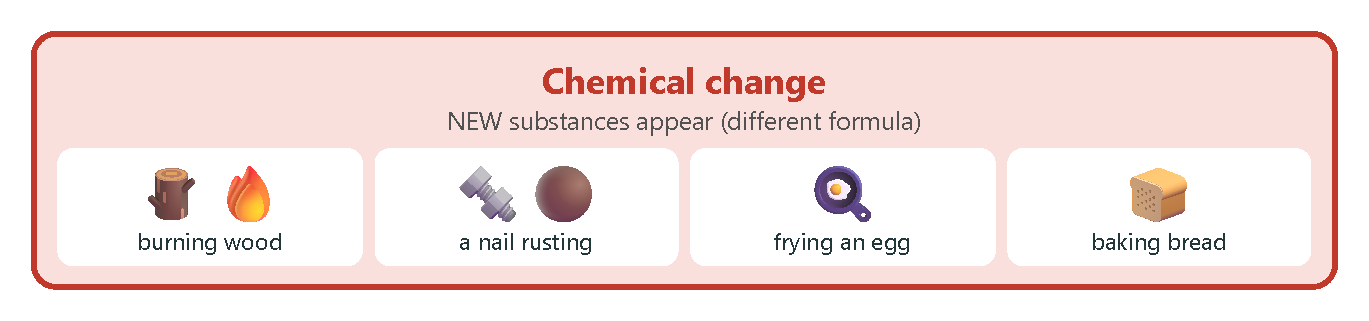
\includegraphics[width=0.85\textwidth]{FigurasSVG/Unit_5_Change_of_Matter/pdf/chemical_change.pdf}
    \caption{Examples of chemical changes: new substances appear.}
    \label{fig:u5_chemical_change}
\end{figure}

\begin{itemize}
    \item \negsubro{Combustion}: when wood, paper or the gas of a cooker burns, it reacts with the oxygen of the air and turns into new substances, such as carbon dioxide, water vapour and ash.
    \item \negsubro{Oxidation}: a nail left outdoors slowly reacts with oxygen and water and becomes covered in rust, a brown substance that is no longer iron.
    \item \negsubro{Cooking food}: when we fry an egg or bake bread, new substances with a different colour, taste and texture are formed; we cannot get the raw egg back.
    \item \negsubro{Decomposition}: a substance breaks down into simpler ones, for example when an electric current splits water into hydrogen and oxygen.
\end{itemize}

\begin{example}
    \begin{itemize}
        \item Passing an electric current through water (\ch{H2O}) produces two new substances: hydrogen (\ch{H2}) and oxygen (\ch{O2}).
        \item Heating a mixture of iron and sulphur produces iron sulphide (\ch{FeS}), a new substance that is \textbf{not} attracted by a magnet, unlike iron.
    \end{itemize}
\end{example}

\subsubsection*{Physical or chemical change?}

To decide whether a change is physical or chemical, we ask: \textbf{is there a new substance at the end?} Figure~\ref{fig:u5_changes_signs} compares both types of change and shows the \textbf{clues} that tell us a chemical change is happening.

\begin{figure}[H]
    \centering
    % [FIGURA ORIGINAL] \includegraphics[width=\textwidth]{Unit_5/changes_signs}
    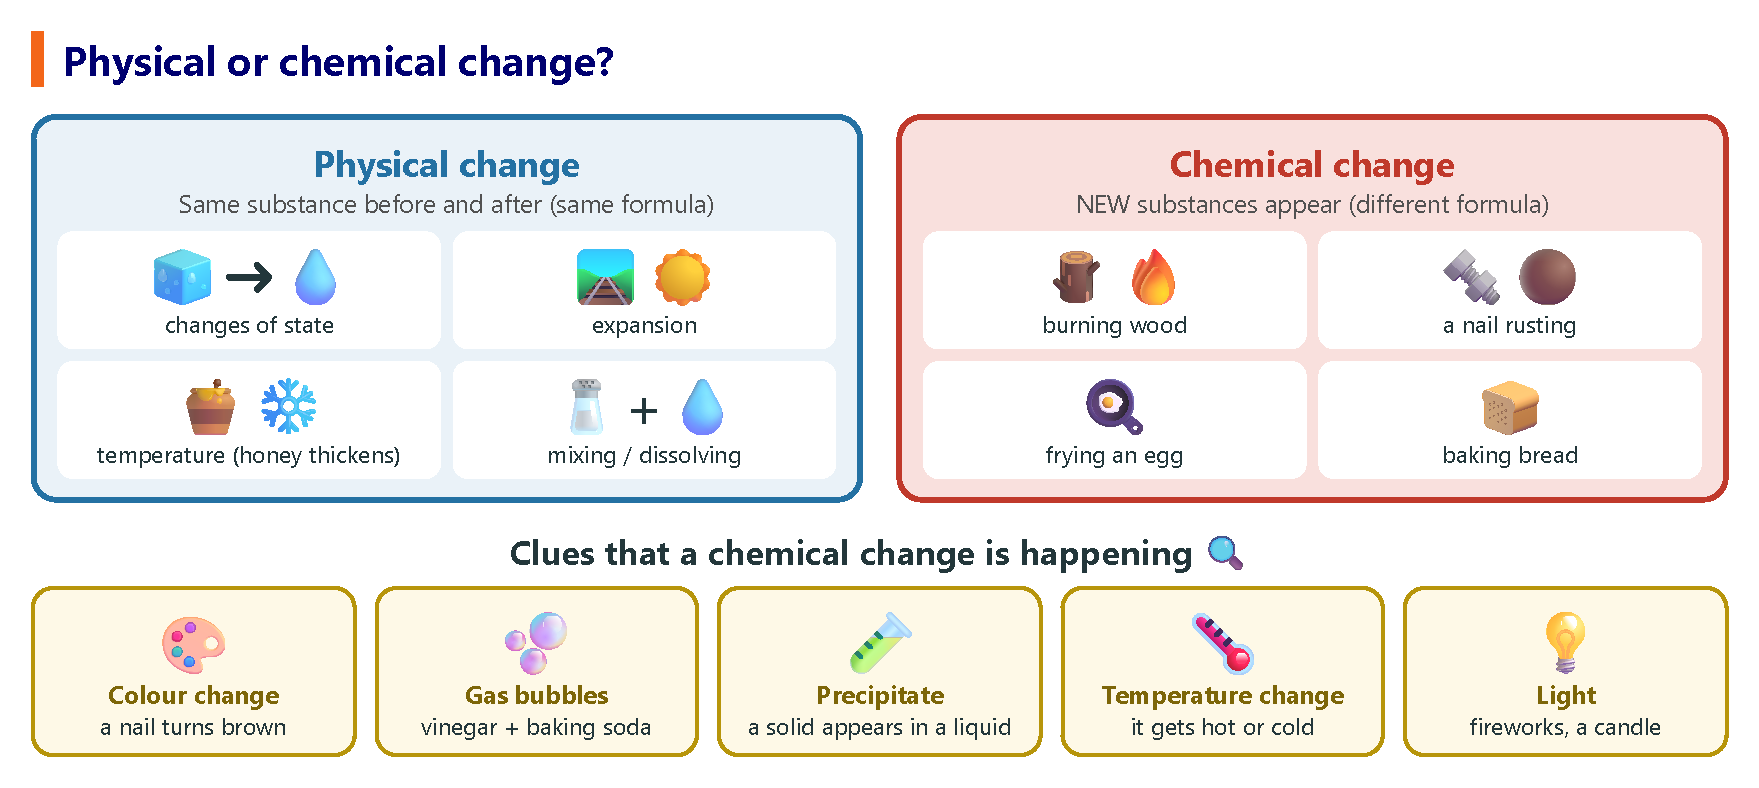
\includegraphics[width=\textwidth]{FigurasSVG/Unit_5_Change_of_Matter/pdf/changes_signs.pdf}
    \caption{Examples of physical and chemical changes, and the clues that tell us a chemical change is happening.}
    \label{fig:u5_changes_signs}
\end{figure}

\begin{impt}
    The clues in the figure suggest a chemical change, but the only \textbf{certain} proof is that new substances, with different properties, have appeared.
\end{impt}

\begin{exercise}
    Classify each transformation as a \textbf{physical} or a \textbf{chemical} change: chopping wood; lighting a candle; burning wood; beating an egg; a key rusting; alcohol evaporating; moulding clay; frying an egg; filtering water with sand; making mayonnaise; iodine subliming.
    \begin{solu}
        \textbf{Physical}: chopping wood, beating an egg, alcohol evaporating, moulding clay, filtering water, making mayonnaise, iodine subliming. \\
        \textbf{Chemical}: lighting a candle, burning wood, a key rusting, frying an egg.
    \end{solu}
\end{exercise}

\begin{exercise}
    Aluminium is obtained from bauxite by passing an electric current through the molten mineral, and later it can be melted down and reused many times. Are these two processes physical or chemical changes?
    \begin{solu}
        Obtaining aluminium from bauxite: \textbf{chemical} (aluminium oxide is transformed into metallic aluminium, a new substance). \\
        Melting aluminium to reuse it: \textbf{physical} (only a change of state); that is why aluminium can be recycled again and again.
    \end{solu}
\end{exercise}

\begin{exercise}
    Is each observation more likely a \textbf{physical} or a \textbf{chemical} change? Ice cubes crack in a warm drink; bubbles appear when vinegar is poured onto baking soda; a nail slowly turns orange-brown outdoors; sugar dissolves in tea; a firework explodes with bright colours.
    \begin{solu}
        Ice cracking: \textbf{physical}. \\
        Vinegar and baking soda: \textbf{chemical} (a gas, \ch{CO2}, is produced). \\
        Rusting nail: \textbf{chemical} (colour change, new substance). \\
        Sugar dissolving: \textbf{physical}. \\
        Firework: \textbf{chemical} (light, heat and new substances).
    \end{solu}
\end{exercise}

\begin{exercise}
    When a solution of silver nitrate is mixed with a solution of sodium chloride, a white solid appears and slowly settles at the bottom of the test tube. What type of change is it, and which clue tells you so?
    \begin{solu}
        A \textbf{chemical change}. The clue is the formation of a \textbf{precipitate} (an insoluble solid appearing inside a liquid).
    \end{solu}
\end{exercise}

%----------------------------------------------------------------------------------------

\section{Separation of the components of a mixture}

The substances in a mixture keep their own properties, so we can separate them using \textbf{physical methods}, which do not change them. We choose the method according to the \textbf{property} that makes the components different (size, density, magnetism, solubility, boiling point\ldots).

\subsection{Separation of heterogeneous mixtures}

\begin{figure}[H]
    \centering
    % [FIGURA ORIGINAL] \includegraphics[width=\textwidth]{Unit_5/separation_hetero}
    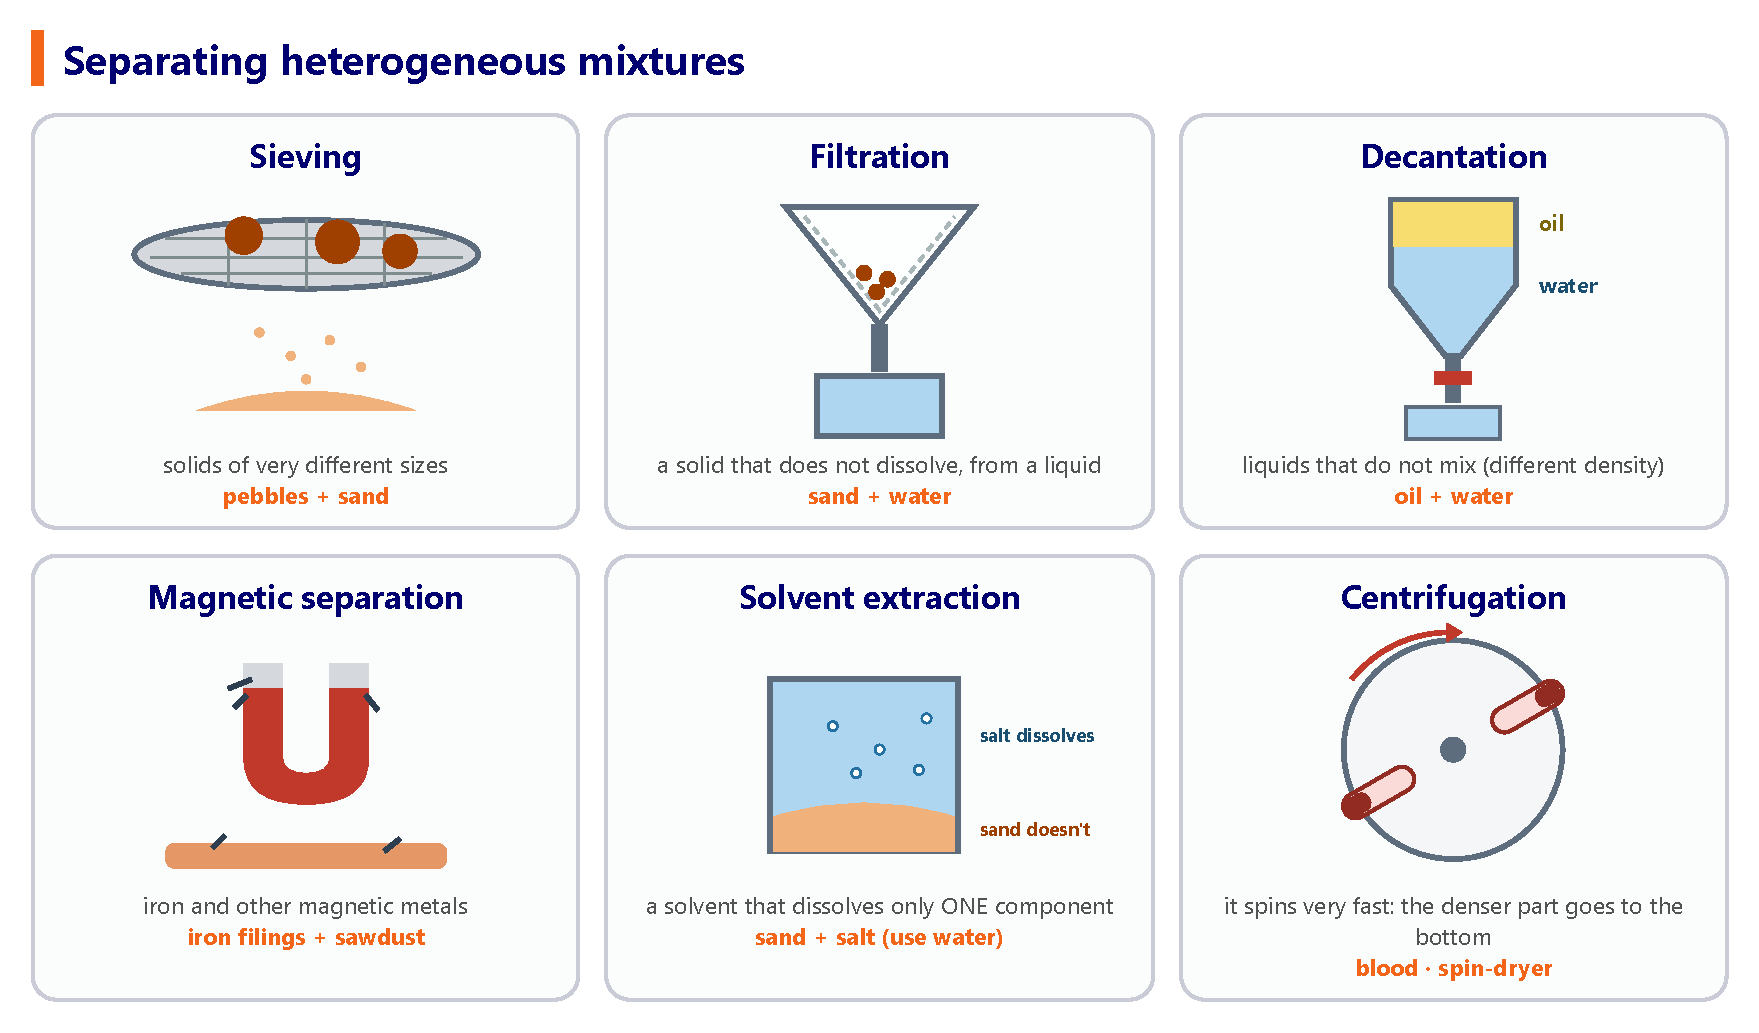
\includegraphics[width=\textwidth]{FigurasSVG/Unit_5_Change_of_Matter/pdf/separation_hetero.pdf}
    \caption{Methods to separate heterogeneous mixtures.}
    \label{fig:u5_separation_hetero}
\end{figure}

\begin{figure}[H]
    \centering
    % [FIGURA ORIGINAL] \includegraphics[width=0.95\textwidth]{Unit_5/filtration}
    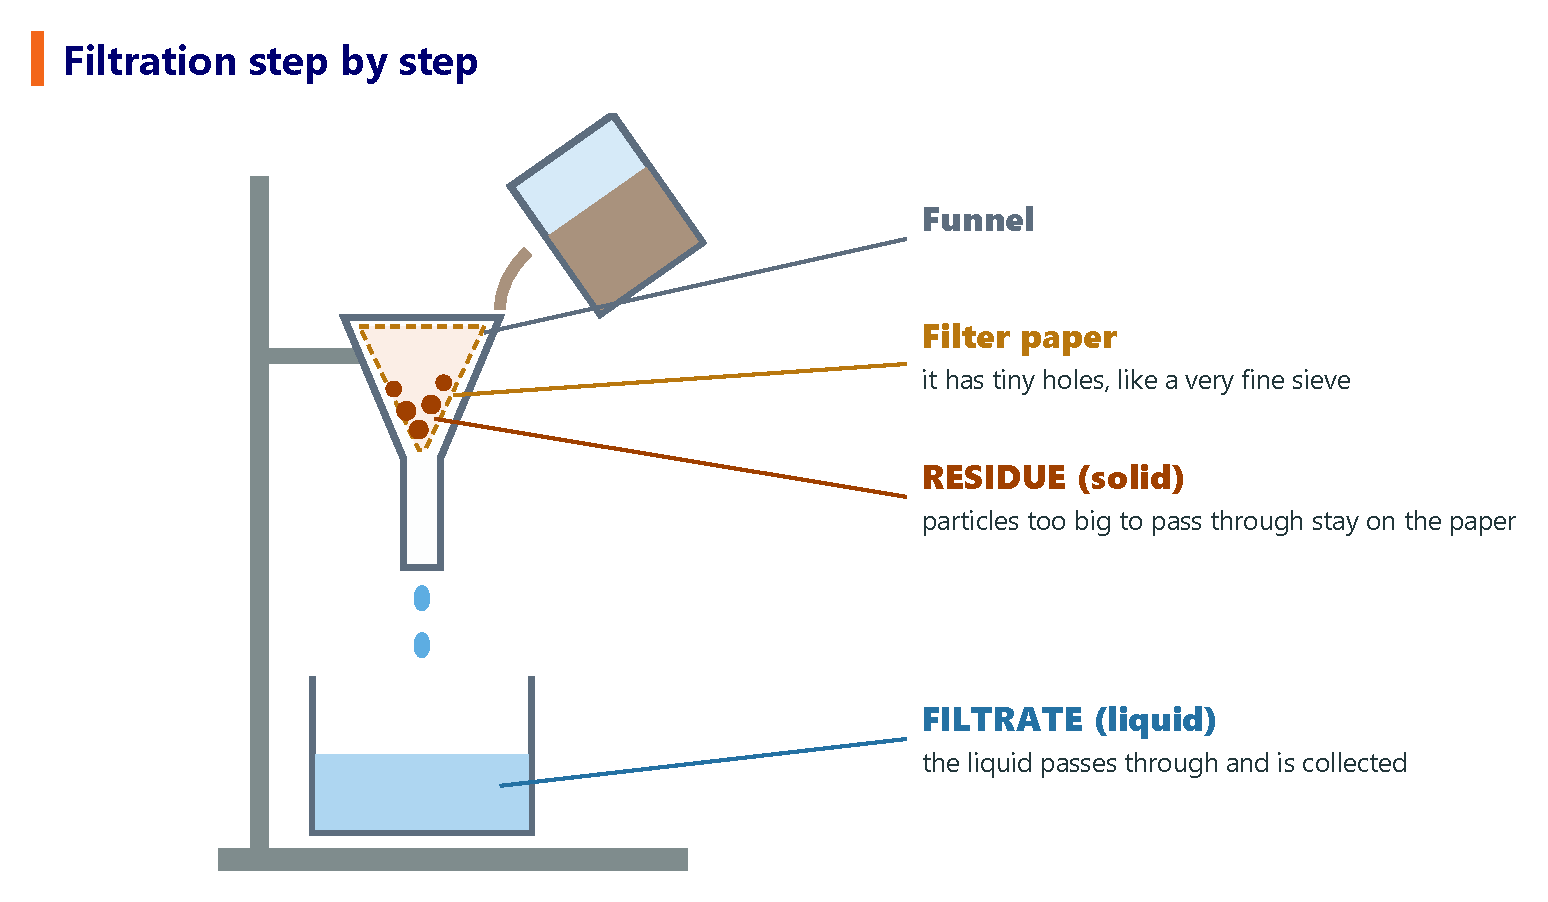
\includegraphics[width=0.95\textwidth]{FigurasSVG/Unit_5_Change_of_Matter/pdf/filtration.pdf}
    \caption{Filtration: the \textit{residue} stays on the paper and the \textit{filtrate} is collected below.}
    \label{fig:u5_filtration}
\end{figure}

Now let us see, \textbf{step by step}, how each of the other methods is carried out in the laboratory.

\begin{figure}[H]
    \centering
    % [FIGURA ORIGINAL] \includegraphics[width=\textwidth]{Unit_5/sieving_steps}
    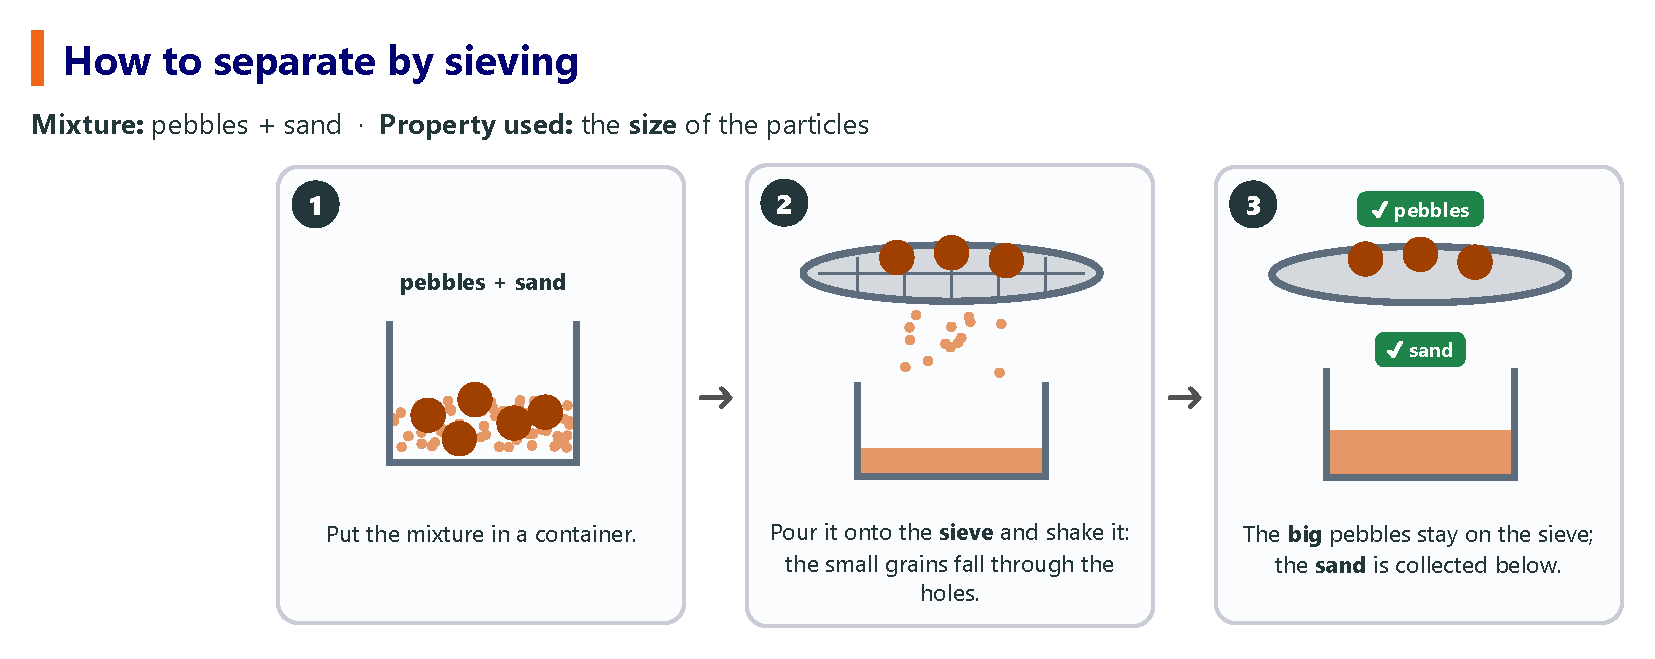
\includegraphics[width=\textwidth]{FigurasSVG/Unit_5_Change_of_Matter/pdf/sieving_steps.pdf}
    \caption{Sieving step by step.}
    \label{fig:u5_sieving_steps}
\end{figure}

\begin{figure}[H]
    \centering
    % [FIGURA ORIGINAL] \includegraphics[width=\textwidth]{Unit_5/decantation_steps}
    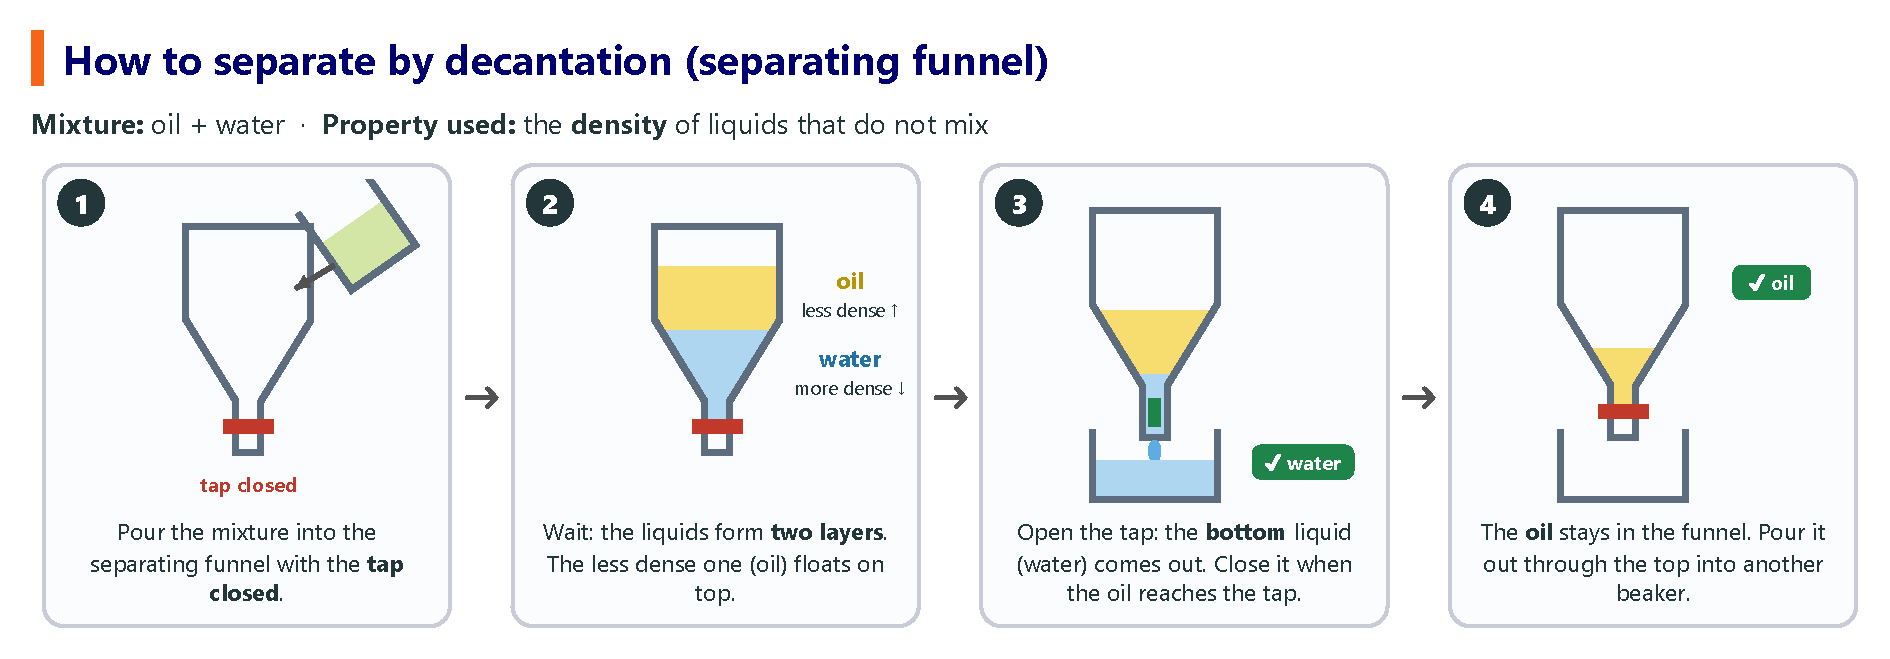
\includegraphics[width=\textwidth]{FigurasSVG/Unit_5_Change_of_Matter/pdf/decantation_steps.pdf}
    \caption{Decantation with a separating funnel, step by step.}
    \label{fig:u5_decantation_steps}
\end{figure}

\begin{figure}[H]
    \centering
    % [FIGURA ORIGINAL] \includegraphics[width=\textwidth]{Unit_5/magnetic_steps}
    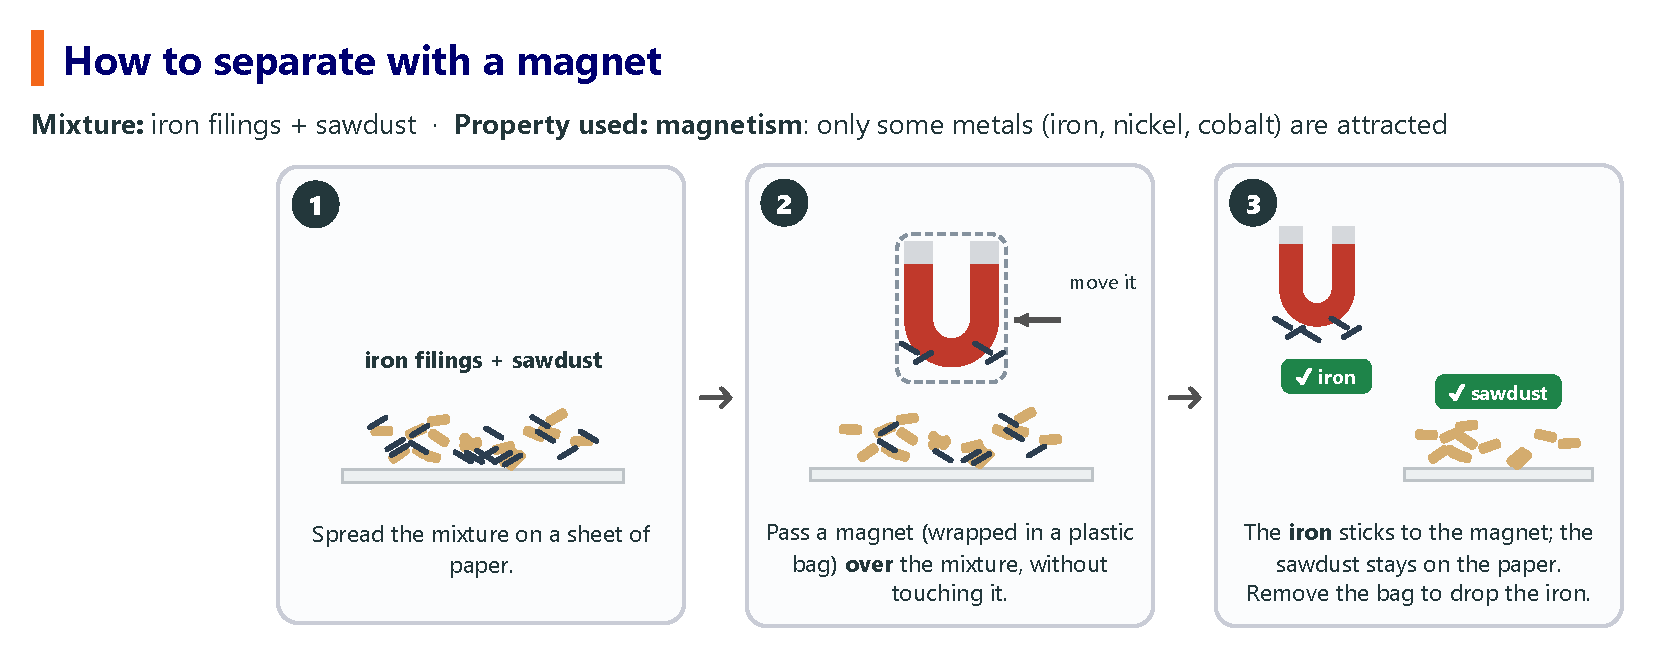
\includegraphics[width=\textwidth]{FigurasSVG/Unit_5_Change_of_Matter/pdf/magnetic_steps.pdf}
    \caption{Magnetic separation step by step.}
    \label{fig:u5_magnetic_steps}
\end{figure}

\begin{figure}[H]
    \centering
    % [FIGURA ORIGINAL] \includegraphics[width=\textwidth]{Unit_5/extraction_steps}
    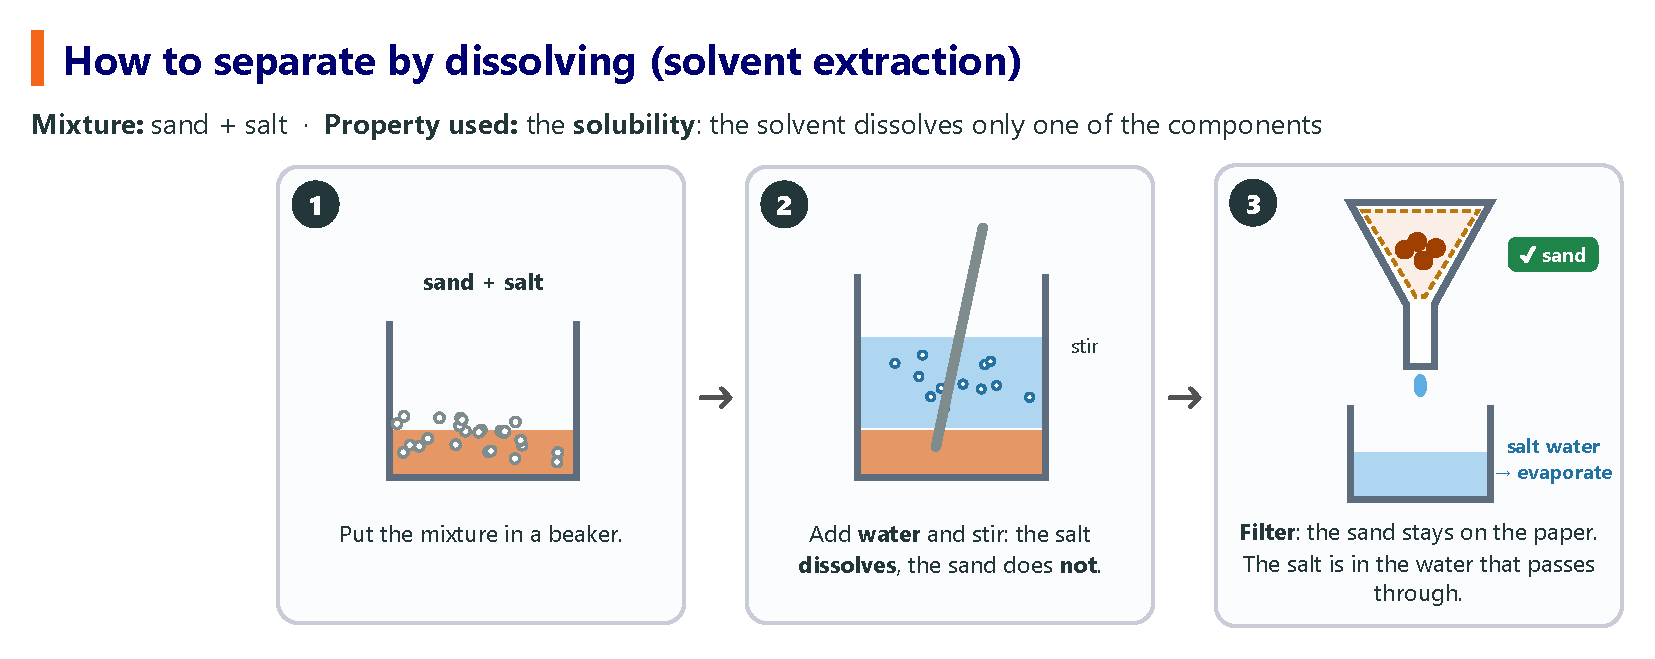
\includegraphics[width=\textwidth]{FigurasSVG/Unit_5_Change_of_Matter/pdf/extraction_steps.pdf}
    \caption{Solvent extraction (separating by dissolving) step by step.}
    \label{fig:u5_extraction_steps}
\end{figure}

\begin{figure}[H]
    \centering
    % [FIGURA ORIGINAL] \includegraphics[width=\textwidth]{Unit_5/centrifugation_steps}
    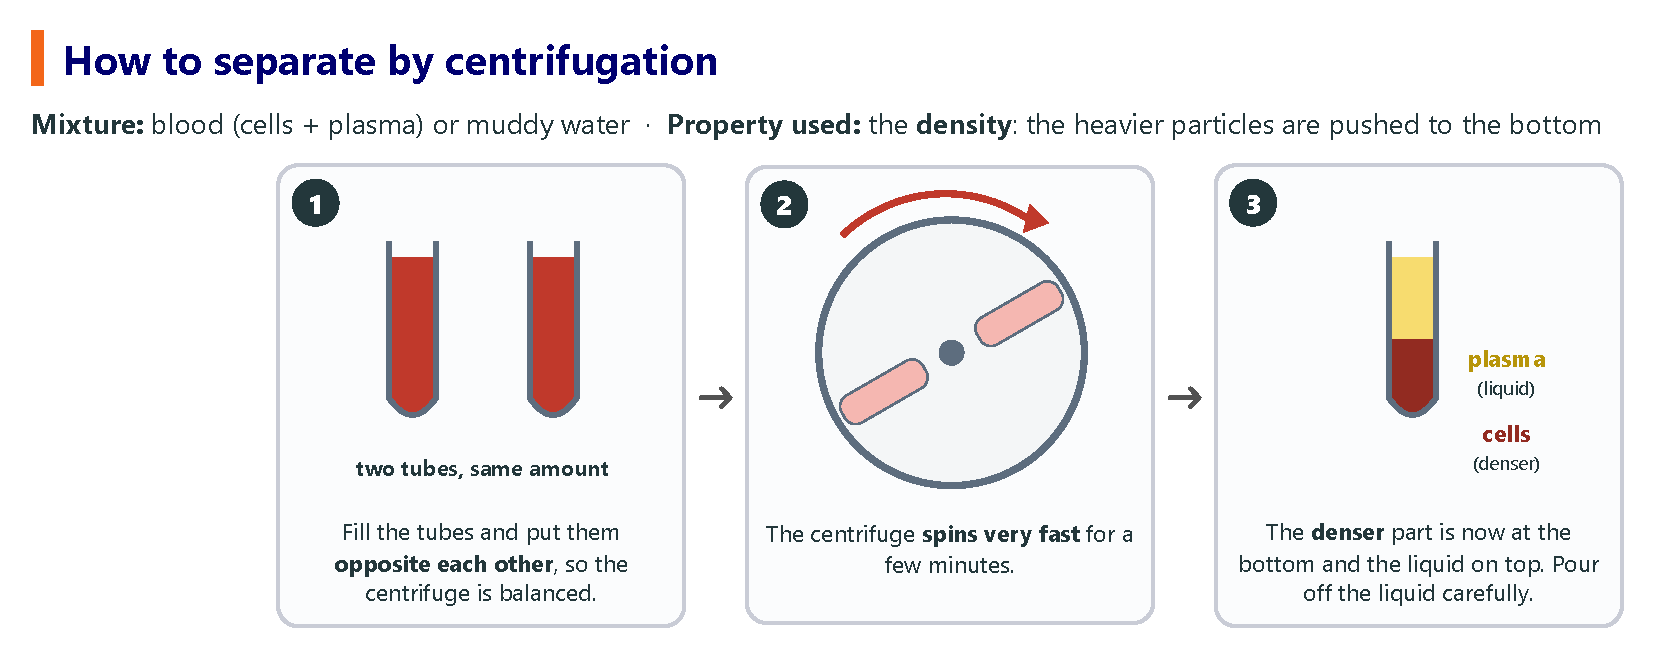
\includegraphics[width=\textwidth]{FigurasSVG/Unit_5_Change_of_Matter/pdf/centrifugation_steps.pdf}
    \caption{Centrifugation step by step.}
    \label{fig:u5_centrifugation_steps}
\end{figure}

\begin{exercise}
    Name the best separation method for each mixture, and justify your choice: gravel and fine sand; iron filings and wood shavings; a salad dressing made of vinegar and olive oil.
    \begin{solu}
        Gravel and sand: \textbf{sieving} (very different sizes). \\
        Iron filings and wood shavings: \textbf{magnetic separation} (only iron is attracted by a magnet). \\
        Vinegar and oil: \textbf{decantation} (liquids that do not mix, with different densities).
    \end{solu}
\end{exercise}

\begin{exercise}
    In a school laboratory, a small sample of muddy water is cleaned with a funnel and filter paper. In a water treatment plant, huge volumes of muddy water are left to stand in large tanks for several hours. Name the technique used in each case, and explain why the plant does not use filter paper.
    \begin{solu}
        Laboratory: \textbf{filtration}. Treatment plant: \textbf{decantation} (sedimentation). Filtering such huge volumes through paper would be far too slow and the filters would block; letting the soil settle under gravity is cheaper and works well for large quantities.
    \end{solu}
\end{exercise}

\subsection{Separation of homogeneous mixtures}

\begin{figure}[H]
    \centering
    % [FIGURA ORIGINAL] \includegraphics[width=\textwidth]{Unit_5/separation_homo}
    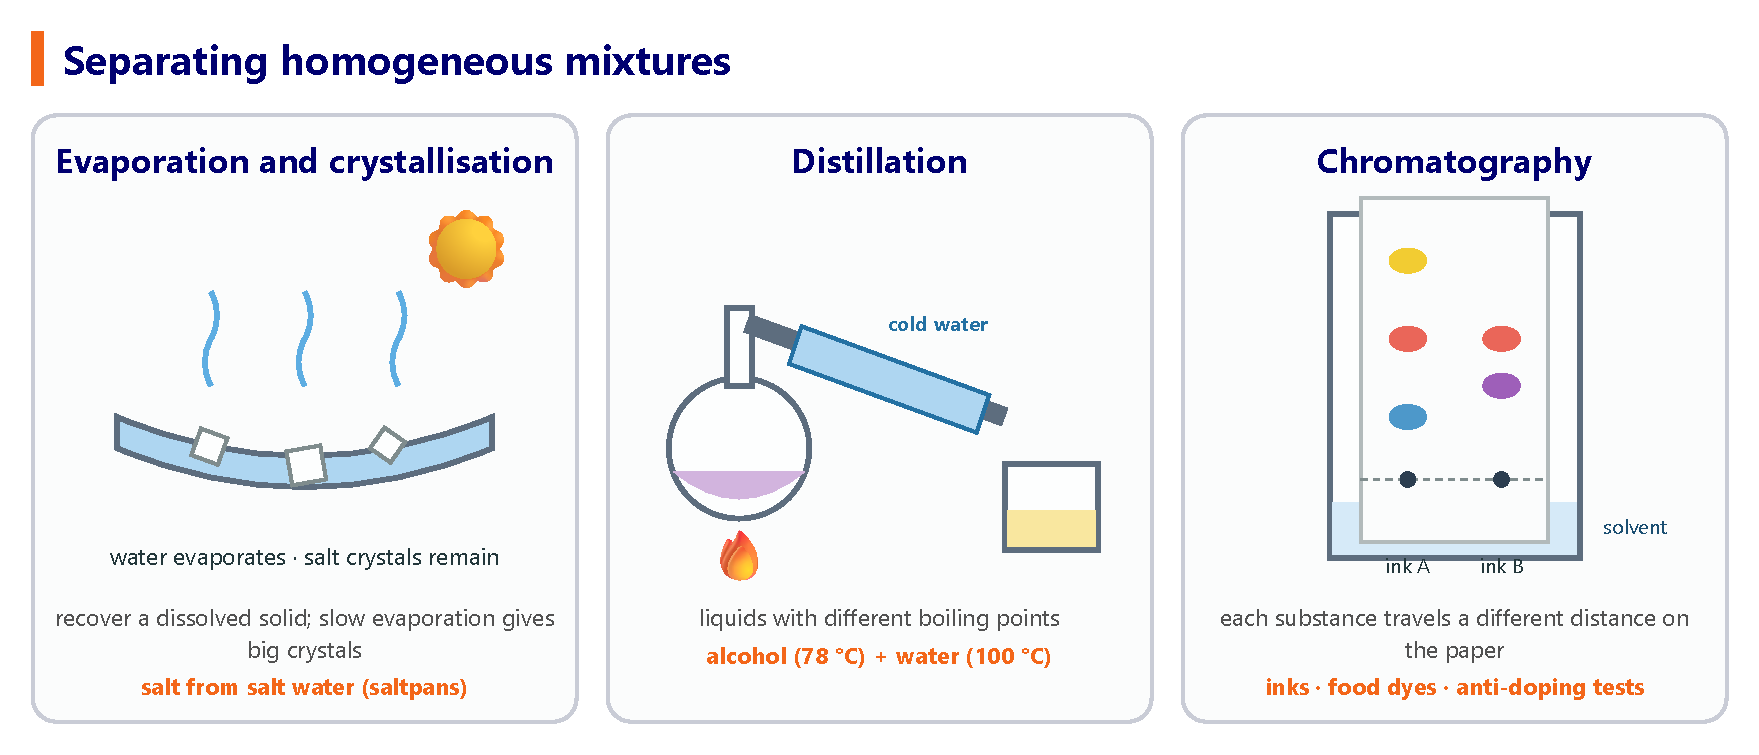
\includegraphics[width=\textwidth]{FigurasSVG/Unit_5_Change_of_Matter/pdf/separation_homo.pdf}
    \caption{Methods to separate homogeneous mixtures.}
    \label{fig:u5_separation_homo}
\end{figure}

\begin{figure}[H]
    \centering
    % [FIGURA ORIGINAL] \includegraphics[width=\textwidth]{Unit_5/distillation}
    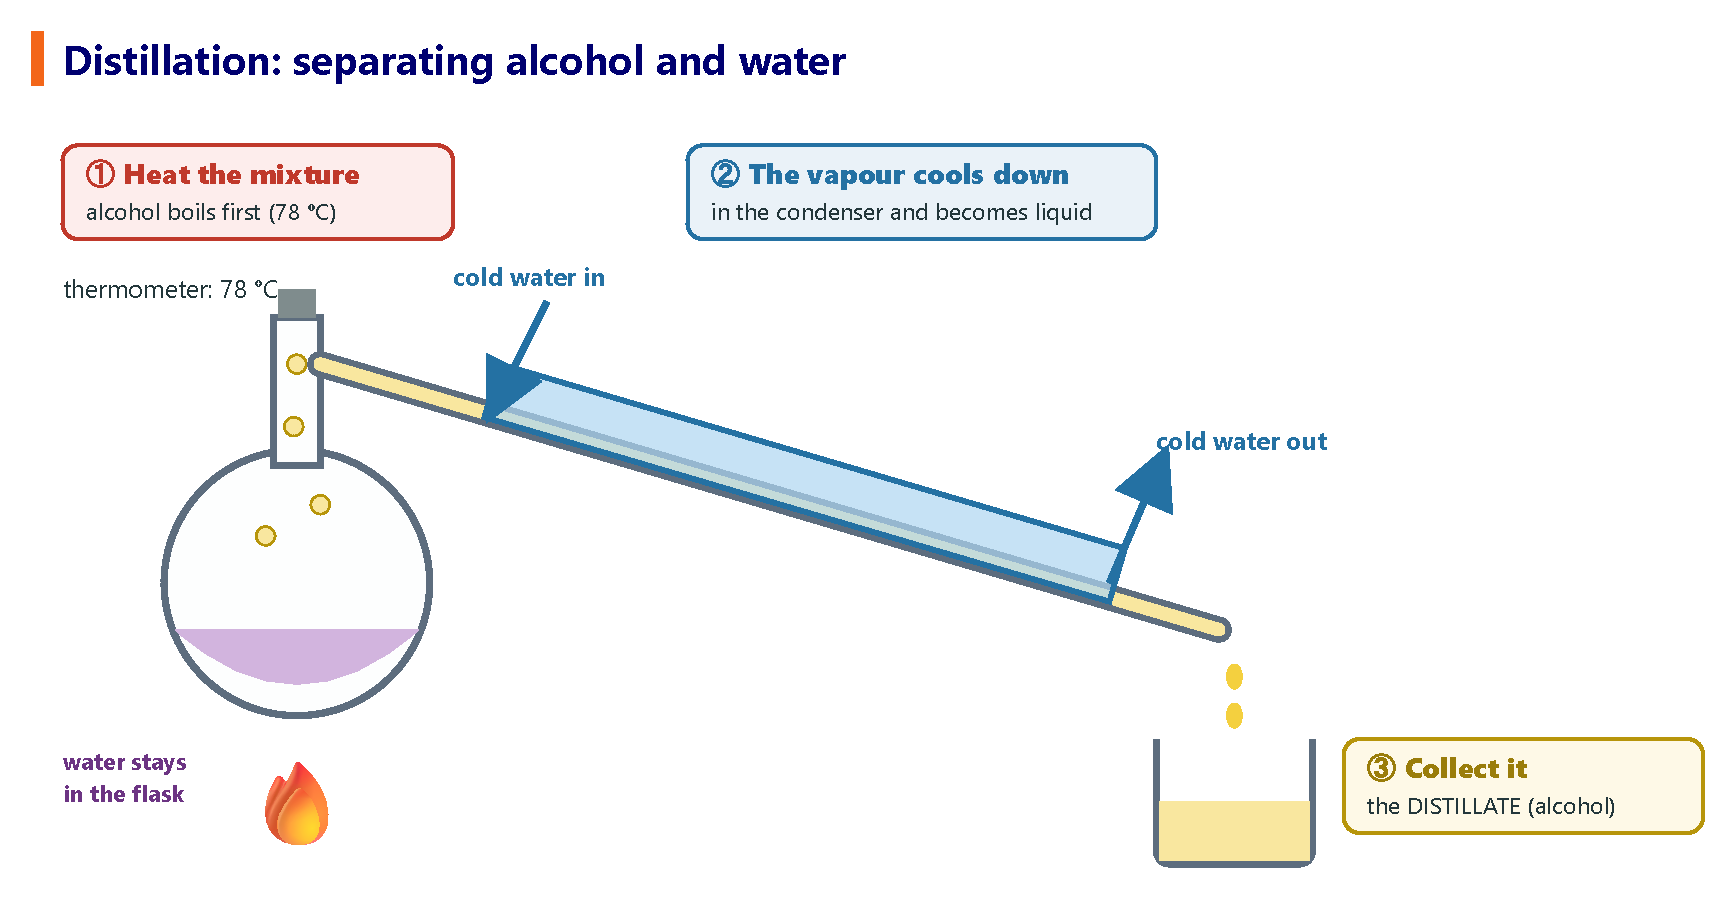
\includegraphics[width=\textwidth]{FigurasSVG/Unit_5_Change_of_Matter/pdf/distillation.pdf}
    \caption{Distillation: the liquid with the lower boiling point evaporates first and is condensed in the condenser.}
    \label{fig:u5_distillation}
\end{figure}

\begin{figure}[H]
    \centering
    % [FIGURA ORIGINAL] \includegraphics[width=\textwidth]{Unit_5/evaporation_steps}
    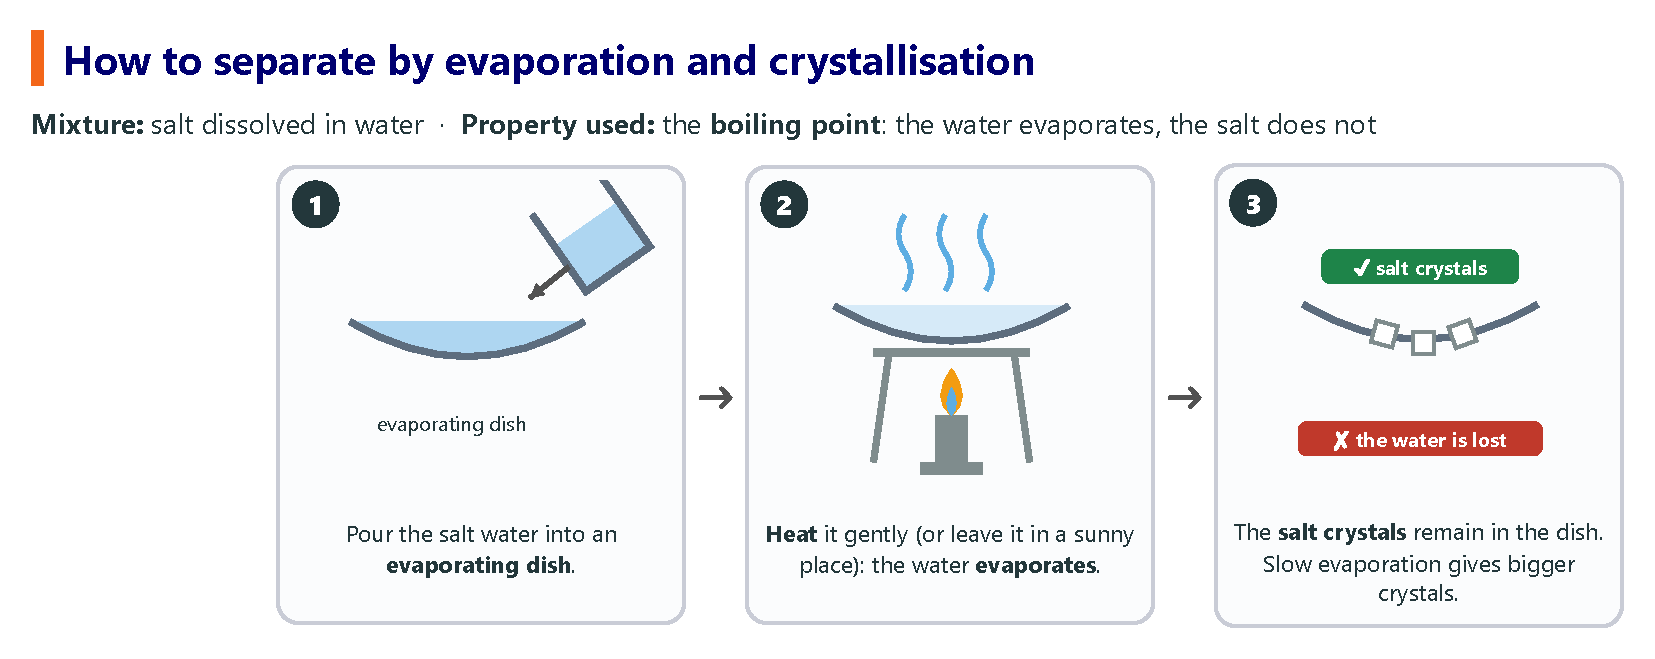
\includegraphics[width=\textwidth]{FigurasSVG/Unit_5_Change_of_Matter/pdf/evaporation_steps.pdf}
    \caption{Evaporation and crystallisation step by step.}
    \label{fig:u5_evaporation_steps}
\end{figure}

\begin{figure}[H]
    \centering
    % [FIGURA ORIGINAL] \includegraphics[width=\textwidth]{Unit_5/chromatography_steps}
    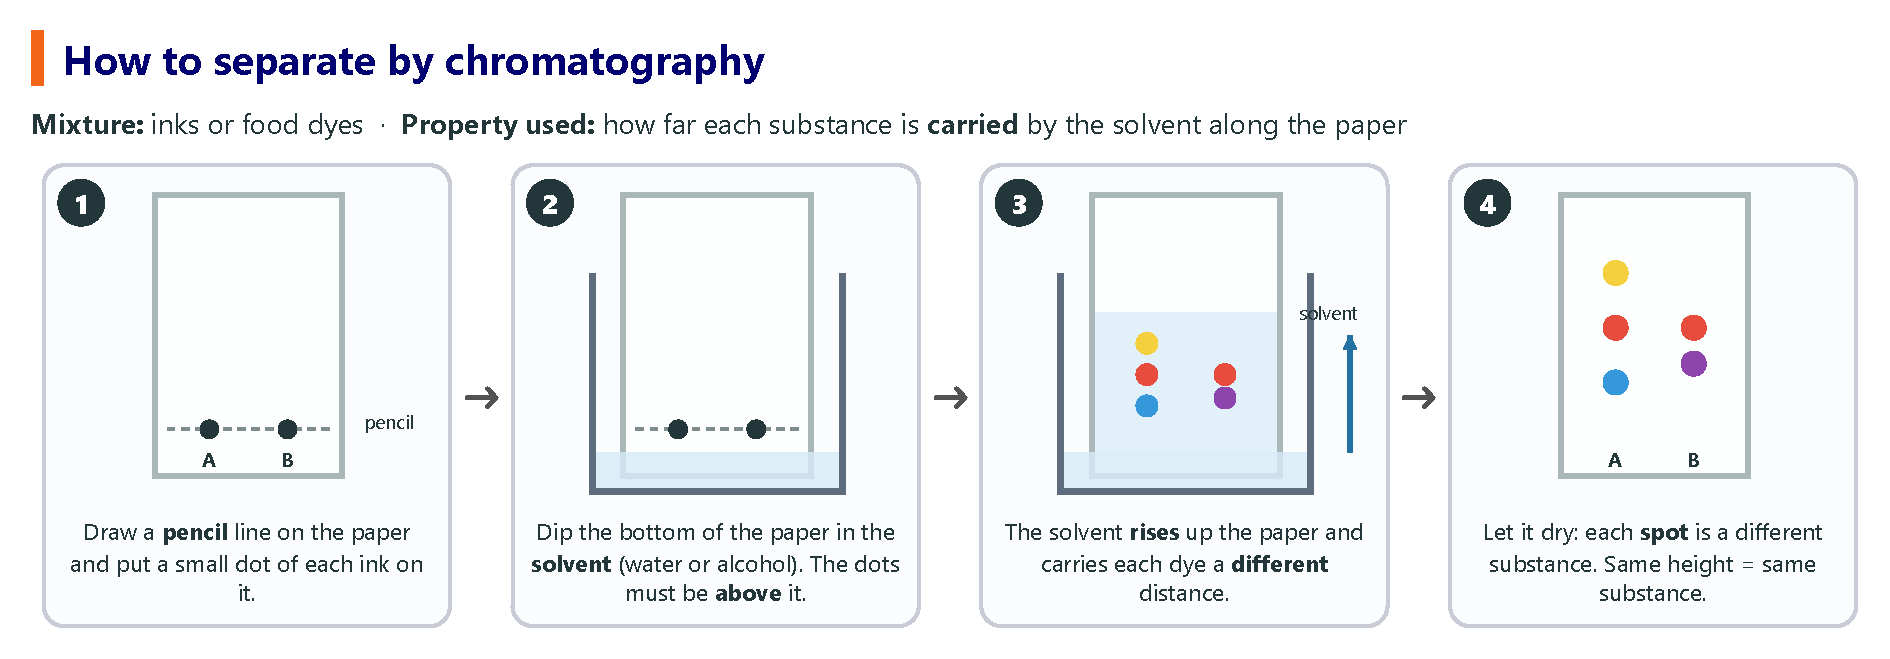
\includegraphics[width=\textwidth]{FigurasSVG/Unit_5_Change_of_Matter/pdf/chromatography_steps.pdf}
    \caption{Paper chromatography step by step.}
    \label{fig:u5_chromatography_steps}
\end{figure}

\begin{didyouknow}
    Many countries with little rain, such as the Canary Islands, get their drinking water from the sea in \textbf{desalination plants}. The seawater is filtered first, and then the salts are removed by distillation or by pushing the water through special membranes.
\end{didyouknow}

\begin{exercise}
    A perfume is a homogeneous mixture of several fragrant substances dissolved in alcohol, each with a different boiling point. Which technique would you use to recover the alcohol, and which property does it use?
    \begin{solu}
        \textbf{Distillation}. It uses the \textbf{different boiling points}: the substance with the lowest boiling point evaporates first and can be condensed and collected separately.
    \end{solu}
\end{exercise}

\begin{exercise}
    A forensic scientist needs to know whether the ink on a note matches the ink from a suspect's pen. Which technique should be used, and how does it allow the two inks to be compared?
    \begin{solu}
        \textbf{Chromatography}. A drop of each ink is placed on filter paper with a solvent; each dye travels a different distance, giving a pattern of coloured spots. If both patterns are the same, the inks are very likely the same.
    \end{solu}
\end{exercise}

\begin{exercise}
    Put these steps of the distillation of a mixture of alcohol and water in the correct order: the alcohol condenses; the mixture reaches the boiling point of alcohol; the alcohol vaporises; the liquid alcohol is collected in another container.
    \begin{solu}
        1.\ The mixture reaches the boiling point of alcohol (\qty{78}{\celsius}). \\
        2.\ The alcohol vaporises. \\
        3.\ The alcohol condenses in the condenser. \\
        4.\ The liquid alcohol is collected in another container.
    \end{solu}
\end{exercise}

\subsection{Applying separation techniques together}

Real mixtures often need \textbf{several} methods, one after another:

\begin{figure}[H]
    \centering
    % [FIGURA ORIGINAL] \includegraphics[width=\textwidth]{Unit_5/separation_steps}
    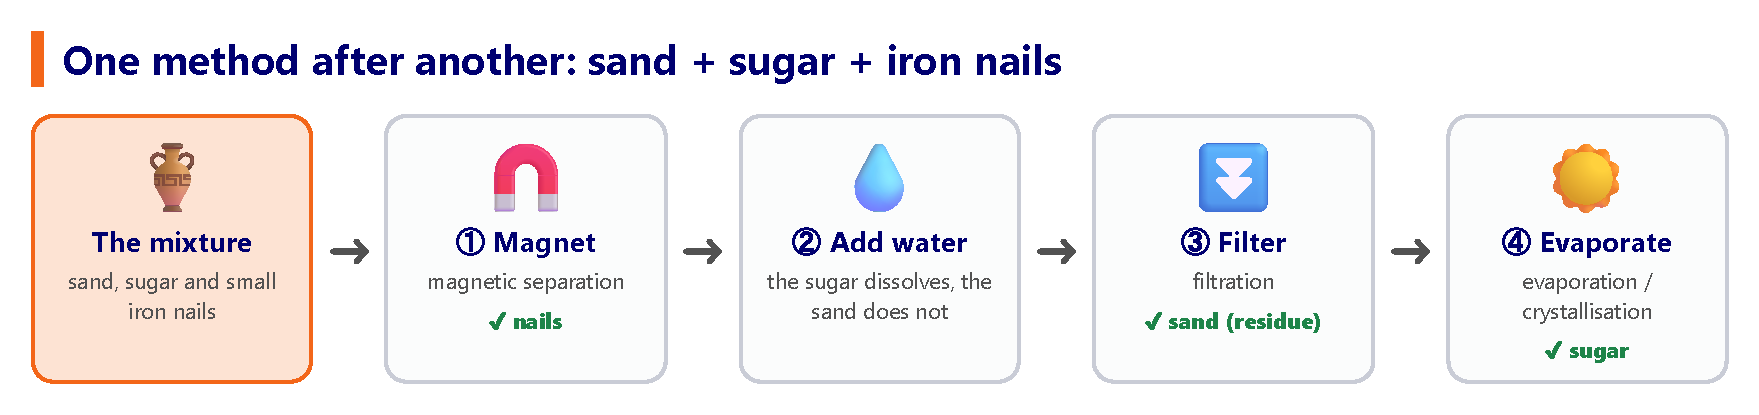
\includegraphics[width=\textwidth]{FigurasSVG/Unit_5_Change_of_Matter/pdf/separation_steps.pdf}
    \caption{Separating a mixture of three components step by step.}
    \label{fig:u5_separation_steps}
\end{figure}

\begin{impt}
    \negsubro{What do I keep and what do I throw away?} After each step the mixture is divided into two parts. Before starting, read the exercise carefully to know \textbf{what you want to obtain}, and after each step decide what to do with each part:
    \begin{itemize}
        \item \textcolor{green!50!black}{\textbf{KEEP}}: it is one of the substances that we want to obtain.
        \item \textcolor{blue!70!black}{\textbf{NEXT STEP}}: it is still a mixture, so we keep separating it.
        \item \textcolor{red!70!black}{\textbf{DISCARD}}: we do not need it (we throw it away or take it to a recycling point).
    \end{itemize}
    Be especially careful when there is a \textbf{solid and a liquid}, as in filtration: the solid that stays on the paper is the \textbf{residue}, and the liquid that passes through is the \textbf{filtrate}. Either of them can be the part we keep, the part that goes on to the next step or the part we throw away: it depends on what we want to obtain.
\end{impt}

\begin{example}
    \textbf{Worked example 1. We have a mixture of sand, salt and iron filings. We want to obtain the three components separately.}
\end{example}

\begin{figure}[H]
    \centering
    % [FIGURA ORIGINAL] \includegraphics[width=\textwidth]{Unit_5/example_sand_salt_iron}
    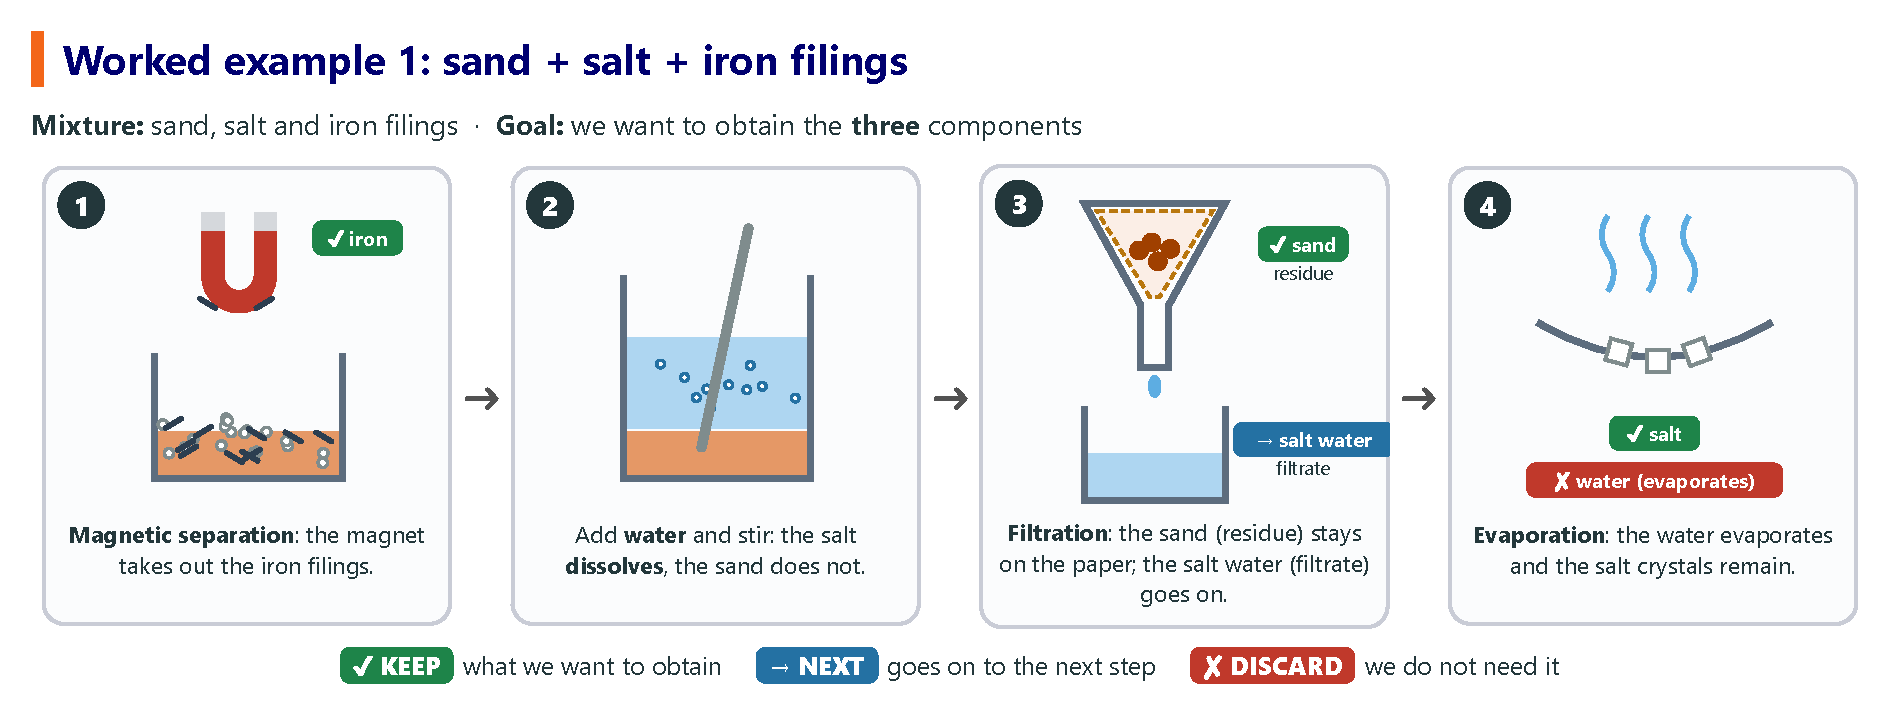
\includegraphics[width=\textwidth]{FigurasSVG/Unit_5_Change_of_Matter/pdf/example_sand_salt_iron.pdf}
    \caption{Worked example 1: separating sand, salt and iron filings.}
    \label{fig:u5_example_sand_salt_iron}
\end{figure}

\begin{enumerate}[label=\numberballmDarkTeal]
    \item \textbf{Magnetic separation.} We pass a magnet over the mixture. Only the iron is attracted. \textcolor{green!50!black}{\textbf{Keep}}: iron filings. \textcolor{blue!70!black}{\textbf{Next step}}: sand + salt.
    \item \textbf{Dissolving.} We add water to the sand and salt and stir. The salt dissolves; the sand does not.
    \item \textbf{Filtration.} We filter the mixture. \textcolor{green!50!black}{\textbf{Keep}}: the sand (\textbf{residue}), which we leave to dry. \textcolor{blue!70!black}{\textbf{Next step}}: the salt water (\textbf{filtrate}).
    \item \textbf{Evaporation.} We heat the salt water in an evaporating dish. \textcolor{green!50!black}{\textbf{Keep}}: the salt crystals. The water evaporates: we \textcolor{red!70!black}{\textbf{lose}} it, but we did not need it.
\end{enumerate}

\begin{tcolorbox}[enhanced, breakable, colback=yellow!6!white, colframe=ocre, boxrule=0.8pt, arc=2mm,
    fonttitle=\sffamily\bfseries, title={How to write it in your notebook}]
    \textbf{Mixture}: sand + salt + iron filings. \quad \textbf{Goal}: obtain the three components.

    \begin{tabular}{@{}p{0.3cm}>{\raggedright\arraybackslash}p{2.9cm}>{\raggedright\arraybackslash}p{3.9cm}>{\raggedright\arraybackslash}p{4.2cm}@{}}
        \toprule
        & \textbf{Method} & \textbf{Why? (property)} & \textbf{Result} \\
        \midrule
        1 & Magnetic separation & iron is attracted by magnets & \textbf{iron} (keep); sand + salt (next) \\
        2 & Dissolve in water & salt is soluble, sand is not & sand + salt water (next) \\
        3 & Filtration & sand does not pass through the paper & residue: \textbf{sand} (keep); filtrate: salt water (next) \\
        4 & Evaporation & water evaporates, salt does not & \textbf{salt} (keep); water (lost) \\
        \bottomrule
    \end{tabular}
\end{tcolorbox}

\begin{example}
    \textbf{Worked example 2. A bucket contains muddy, oily water: sand, oil and water. We want to obtain clean water.}
\end{example}

\begin{figure}[H]
    \centering
    % [FIGURA ORIGINAL] \includegraphics[width=\textwidth]{Unit_5/example_sand_oil_water}
    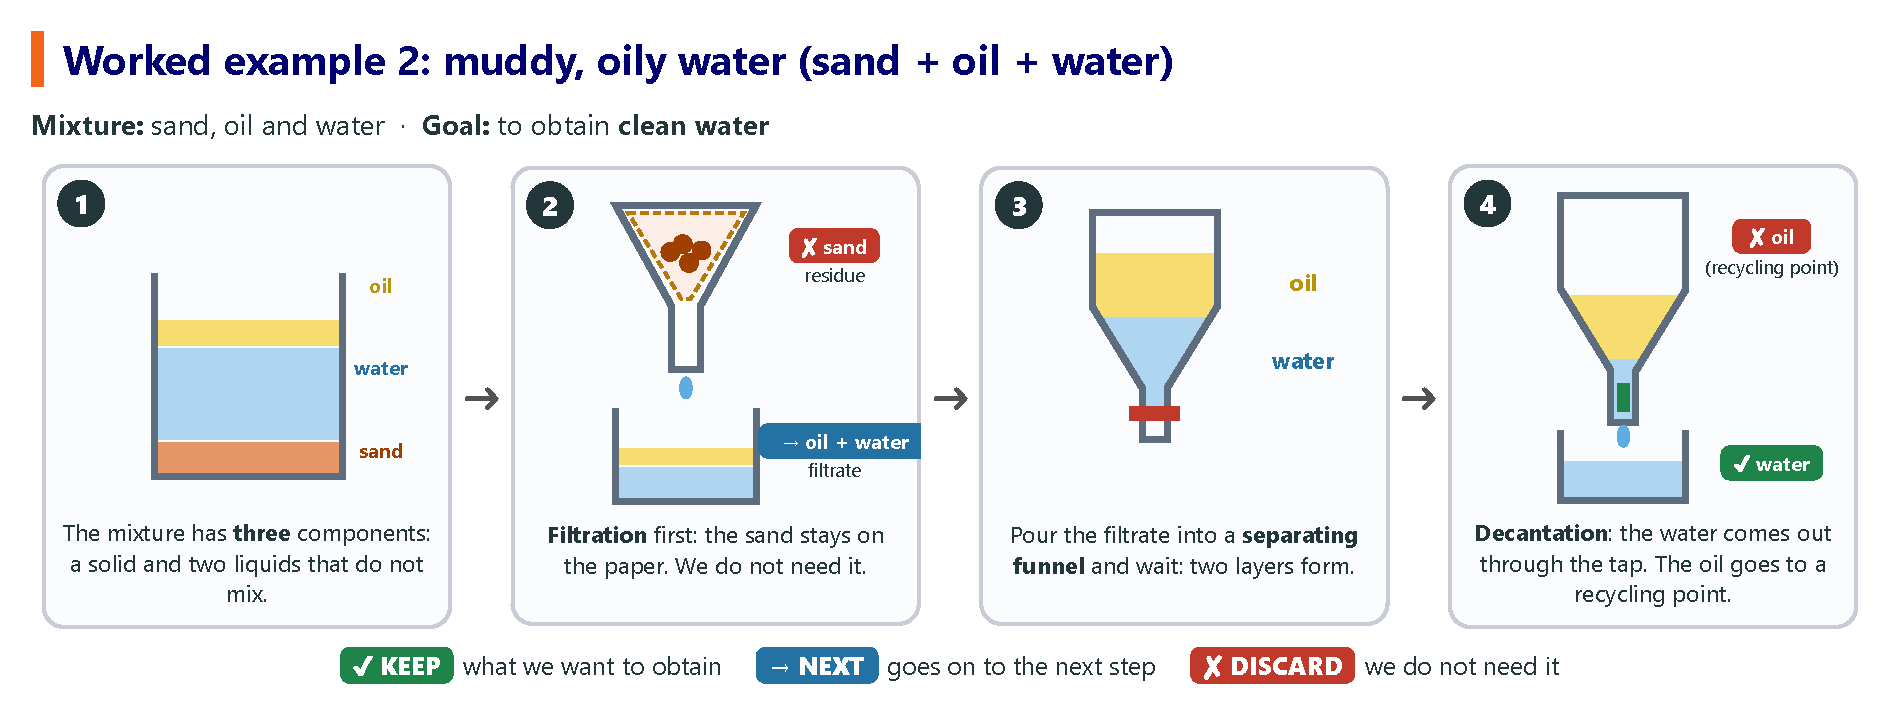
\includegraphics[width=\textwidth]{FigurasSVG/Unit_5_Change_of_Matter/pdf/example_sand_oil_water.pdf}
    \caption{Worked example 2: obtaining clean water from a mixture of sand, oil and water.}
    \label{fig:u5_example_sand_oil_water}
\end{figure}

\begin{enumerate}[label=\numberballmDarkTeal]
    \item We look at the mixture: one solid (sand) and two liquids that do not mix (oil and water).
    \item \textbf{Filtration first}, so that the sand does not block the tap of the separating funnel. \textcolor{red!70!black}{\textbf{Discard}}: the sand (\textbf{residue}), because we only want the water. \textcolor{blue!70!black}{\textbf{Next step}}: oil + water (\textbf{filtrate}).
    \item We pour the filtrate into a \textbf{separating funnel} and wait until two layers form: the oil, less dense, on top; the water, more dense, at the bottom.
    \item \textbf{Decantation.} We open the tap and let the water out, closing it when the oil reaches the tap. \textcolor{green!50!black}{\textbf{Keep}}: the clean water. \textcolor{red!70!black}{\textbf{Discard}}: the oil, which must \textbf{never} be poured down the sink: we take it to a recycling point.
\end{enumerate}

\begin{tcolorbox}[enhanced, breakable, colback=yellow!6!white, colframe=ocre, boxrule=0.8pt, arc=2mm,
    fonttitle=\sffamily\bfseries, title={How to write it in your notebook}]
    \textbf{Mixture}: sand + oil + water. \quad \textbf{Goal}: obtain clean water.

    \begin{tabular}{@{}p{0.3cm}>{\raggedright\arraybackslash}p{2.9cm}>{\raggedright\arraybackslash}p{3.9cm}>{\raggedright\arraybackslash}p{4.2cm}@{}}
        \toprule
        & \textbf{Method} & \textbf{Why? (property)} & \textbf{Result} \\
        \midrule
        1 & Filtration & sand does not pass through the paper & residue: sand (discard); filtrate: oil + water (next) \\
        2 & Decantation (separating funnel) & oil and water do not mix and have different densities & \textbf{water} (keep); oil (recycling point) \\
        \bottomrule
    \end{tabular}
\end{tcolorbox}

\begin{marker}
    In your notebook, always write the steps \textbf{in order} and, for each one: the \textbf{name of the method}, the \textbf{property} that makes it work, and what happens to \textbf{each part} (keep, next step or discard).
\end{marker}

\begin{exercise}
    A mixture of sand, water and oil needs to be separated. You have a funnel, filter paper, beakers, stands and a separating funnel.
    \begin{enumerate}[label=\letraminuscula]
        \item Which two separation methods should be used?
        \item Which one should be done first? Why?
    \end{enumerate}
    \begin{solu}
        \begin{enumerate}[label=\alph*)]
            \item \textbf{Filtration} (to remove the sand) and \textbf{decantation} (to separate the oil from the water).
            \item \textbf{Filtration} first: otherwise the sand could block the tap of the separating funnel.
        \end{enumerate}
    \end{solu}
\end{exercise}

\begin{exercise}
    Wastewater treatment plants first remove large solid waste with grids, then let sand and grit settle at the bottom of large tanks, and finally use bacteria to purify the water. Name the separation technique used in each of the first two steps.
    \begin{solu}
        Grids: \textbf{sieving}. Letting sand settle: \textbf{decantation}.
    \end{solu}
\end{exercise}

\begin{exercise}
    A laboratory needs to separate the cells in a blood sample quickly. Which technique should be used, and why is it faster than decantation?
    \begin{solu}
        \textbf{Centrifugation}. The sample spins very fast, and this pushes the denser particles to the bottom much faster than gravity alone.
    \end{solu}
\end{exercise}

\begin{exercise}
    Seawater sometimes contains, besides dissolved salts, floating seaweed and suspended sand. Design a step-by-step procedure to obtain both drinking water and solid salt from it.
    \begin{solu}
        \begin{enumerate}
            \item \textbf{Filtration}: remove the seaweed and the sand.
            \item \textbf{Distillation}: the water evaporates and is condensed and collected (drinking water).
            \item \textbf{Evaporation/crystallisation}: let the concentrated salty water left behind evaporate completely to obtain salt crystals.
        \end{enumerate}
    \end{solu}
\end{exercise}

%----------------------------------------------------------------------------------------

\section*{Summary}

\begin{itemize}
    \item \textbf{Physical change}: no new substances (changes of state, temperature, expansion, mixing). \textbf{Chemical change}: new substances appear. Clues: colour change, gas, precipitate, temperature change, light.
    \item \textbf{Separating heterogeneous mixtures}: sieving, filtration, decantation, magnetic separation, solvent extraction, centrifugation.
    \item \textbf{Separating homogeneous mixtures}: evaporation/crystallisation, distillation, chromatography. Several methods are often used one after another.
\end{itemize}

\section{Vocabulary}

\begin{vocabulary}[Physical change]
    A change in matter that does not affect its nature. \newline
    \textbf{Translation to Spanish}: Cambio físico
\end{vocabulary}

\begin{vocabulary}[Chemical change]
    A change that transforms matter into new substances. \newline
    \textbf{Translation to Spanish}: Cambio químico
\end{vocabulary}

\begin{vocabulary}[Precipitate]
    An insoluble solid that appears inside a liquid, often as a sign of a chemical change. \newline
    \textbf{Translation to Spanish}: Precipitado
\end{vocabulary}

\begin{vocabulary}[Sieving]
    Separating solids of different sizes with a sieve. \newline
    \textbf{Translation to Spanish}: Tamizado
\end{vocabulary}

\begin{vocabulary}[Filtration]
    Separation method for a solid that does not dissolve in a liquid. \newline
    \textbf{Translation to Spanish}: Filtración
\end{vocabulary}

\begin{vocabulary}[Decantation]
    Separation method for immiscible liquids of different densities. \newline
    \textbf{Translation to Spanish}: Decantación
\end{vocabulary}

\begin{vocabulary}[Magnetic separation]
    Separating magnetic metals, such as iron, from a mixture with a magnet. \newline
    \textbf{Translation to Spanish}: Separación magnética
\end{vocabulary}

\begin{vocabulary}[Centrifugation]
    Separation method that uses centrifugal force to speed up the sedimentation of a solid suspended in a liquid. \newline
    \textbf{Translation to Spanish}: Centrifugación
\end{vocabulary}

\begin{vocabulary}[Crystallisation]
    Obtaining a dissolved solid as crystals by letting the solvent evaporate slowly. \newline
    \textbf{Translation to Spanish}: Cristalización
\end{vocabulary}

\begin{vocabulary}[Distillation]
    Separation method for miscible liquids with different boiling points. \newline
    \textbf{Translation to Spanish}: Destilación
\end{vocabulary}

\begin{vocabulary}[Chromatography]
    Separation method based on different affinity for a surface. \newline
    \textbf{Translation to Spanish}: Cromatografía
\end{vocabulary}
